\documentclass[t, notes]{beamer}

\usepackage{wrapfig}
\usepackage{float}
% For tabs in verbatim
\usepackage{fancyvrb}

% set fonts
\usefonttheme{professionalfonts} % using non standard fonts for beamer
\usepackage{txfonts,mathptmx}

% set indend spacing for first and second level indentation
\setlength{\leftmargini}{0.5cm}
\setlength{\leftmarginii}{0.5cm}
\setlength{\leftmarginiii}{0.5cm}

% Set circles for bullets 
\setbeamertemplate{itemize items}[circle]

% colors
\usepackage{xcolor}

% multiple columns
\usepackage{multicol}

% todo lists
\usepackage{pifont}
\usepackage{amssymb}

% increase space between text and frame name
\addtobeamertemplate{frametitle}{}{\vspace{0.5em}}

%Information to be included in the title page:
\title{Verilog Introduction}
\author{Nikola Petrovic}
\institute{University of Belgrade, School of Electrical Engineering}
\date{2022}



\begin{document}

\frame{\titlepage}

%%%%%%%%%%%%%%%%%%%%%%%%%%%%%%%%%%%%%%%%%%%%%%%%%%%%%%%%%%%%
\begin{frame}
\frametitle{Module Objective}

In this module we will use Verilog to describe a simple design.
\newline

\textbf{Topics}

\begin{itemize}
\item Describing design modules
\item Representing hierarchy
\item Describing module behavior
\item Synchronizing module behaviors
\item Communicating between behaviors
\item Rules for identifiers, comments, white space
\item Configuring and compiling a design
\end{itemize}

\end{frame}

%%%%%%%%%%%%%%%%%%%%%%%%%%%%%%%%%%%%%%%%%%%%%%%%%%%%%%%%%%%%
\begin{frame}[fragile]
\frametitle{Describing Design Modules}

\begin{enumerate}
\item We need to start with \textcolor{red}{module} keyword
\item \textcolor{purple}{Describe module interface}
\item \textcolor{brown}{Describe module behavior}
\item End with \textcolor{red}{endmodule} keyword
\end{enumerate}

In Verilog-2001 we can write:
\newline

\begin{Verbatim}[commandchars=\\\{\}, tabsize=2]
\textcolor{purple}{module} halfadd (
	\textcolor{purple}{input} a, b,
	\textcolor{purple}{output} sum, carry
);
	\textcolor{purple}{assign} sum   = a ^ b;
	\textcolor{purple}{assign} carry = a & b;
\textcolor{purple}{endmodule}
\end{Verbatim}

\end{frame}

%%%%%%%%%%%%%%%%%%%%%%%%%%%%%%%%%%%%%%%%%%%%%%%%%%%%%%%%%%%%
\begin{frame}
\frametitle{Creating Hierarchy}

\begin{itemize}
\item We need to declare local nets and variables
\item Instantiate module and connect its ports to the local nets and variables
\item We can connect an instance of a module using:
\begin{itemize}
	\item Named port connection.
	\item Ordered port connection.
\end{itemize}
\item We will be connecting two half-adders together:
\end{itemize}

\begin{figure}[H!]
    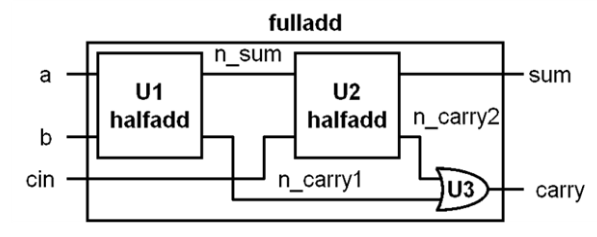
\includegraphics[width=0.5\textwidth]{img/03_fulladd.png}
\end{figure}

\end{frame}

%%%%%%%%%%%%%%%%%%%%%%%%%%%%%%%%%%%%%%%%%%%%%%%%%%%%%%%%%%%%
\begin{frame}[fragile]
\frametitle{Named port connection}
\begin{multicols}{2}
{\scriptsize%
\begin{Verbatim}[commandchars=\\\{\}, tabsize=2]
\textcolor{purple}{module} fulladd(
    \textcolor{blue}{input} a, b, cin,
    \textcolor{blue}{output} sum, carry
);
    \textcolor{blue}{wire} w_sum, w_carry1, w_carry2;
    \textcolor{blue}{halfadd U1}(
        .a(a),
        .b(b),
        .sum(w_sum),
        .carry(w_carry1)
    );
    \textcolor{blue}{halfadd U2}(
        .a(w_sum),
        .b(cin),
        .sum(sum),
        .carry(w_carry2)
    );
    \textcolor{blue}{or U3}(
        carry, 
        w_carry2,
        w_carry1
    );
\textcolor{purple}{endmodule}
\end{Verbatim}
}
\columnbreak
\begin{figure}[H!]
	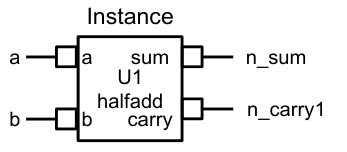
\includegraphics[width=0.35\textwidth]{img/03_inst.png}
\end{figure}
\begin{figure}[H!]
    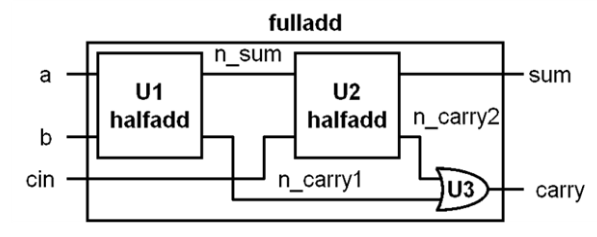
\includegraphics[width=0.35\textwidth]{img/03_fulladd.png}
\end{figure}
\end{multicols}
\end{frame}

%%%%%%%%%%%%%%%%%%%%%%%%%%%%%%%%%%%%%%%%%%%%%%%%%%%%%%%%%%%%
\begin{frame}[fragile]
\frametitle{Ordered port connection}
\begin{multicols}{2}
{\scriptsize%
\begin{Verbatim}[commandchars=\\\{\}, tabsize=2]
\textcolor{purple}{module} fulladd(
    \textcolor{blue}{input} a, b, cin,
    \textcolor{blue}{output} sum, carry
);
    \textcolor{blue}{wire} w_sum, w_carry1, w_carry2;
    \textcolor{blue}{halfadd U1}(
        a,
        b,
        w_sum,
        w_carry1
    );
    \textcolor{blue}{halfadd U2}(
        w_sum,
        cin,
        sum,
        w_carry2
    );
    \textcolor{blue}{or U3}(
        carry, 
        w_carry2,
        w_carry1
    );
\textcolor{purple}{endmodule}
\end{Verbatim}
}
\columnbreak
\begin{figure}[H!]
	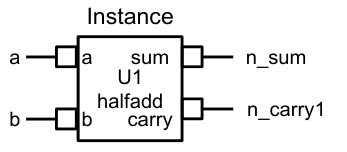
\includegraphics[width=0.35\textwidth]{img/03_inst.png}
\end{figure}
\begin{figure}[H!]
    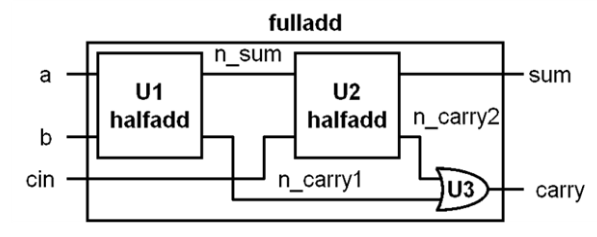
\includegraphics[width=0.35\textwidth]{img/03_fulladd.png}
\end{figure}
\end{multicols}
\end{frame}

%%%%%%%%%%%%%%%%%%%%%%%%%%%%%%%%%%%%%%%%%%%%%%%%%%%%%%%%%%%%
\begin{frame}[fragile]
\frametitle{Describing Module Behavior With Procedural Blocks}

\begin{multicols}{2}
\begin{itemize}
\item Procedural blocks start with:
\begin{itemize}
	\item \textcolor{purple}{always}
	\begin{itemize}
		\item Synthesizable construct
		\item Executes at the start of simulation
		\item Execution blocks and unblocks in accordance with timing controls
		\item When at end, loops back to beginning
	\end{itemize}
\end{itemize}
\begin{itemize}
	\item \textcolor{purple}{initial}
	\begin{itemize}
		\item Non-synthesizable  or Testbench construct
		\item Executes at the start of simulation
		\item Execution blocks and unblocks in accordance with timing controls
		\item When at end, terminates
	\end{itemize}
\end{itemize}
\end{itemize}

\columnbreak
{\footnotesize%
\begin{Verbatim}[commandchars=\\\{\}, tabsize=2]
\textcolor{purple}{always} @ (a or b or select)
\textcolor{blue}{begin}
	\textcolor{purple}{if} (select == 1)
		op = b;
	\textcolor{purple}{else}
		op = a;
\textcolor{blue}{end}



\textcolor{purple}{initial}
\textcolor{blue}{begin}
	a = 1;
	b = 0;
\textcolor{blue}{end}
\end{Verbatim}
}
\end{multicols}
\end{frame}

%%%%%%%%%%%%%%%%%%%%%%%%%%%%%%%%%%%%%%%%%%%%%%%%%%%%%%%%%%%%
\begin{frame}[fragile]
\frametitle{Describing Module Behavior With Procedural Blocks}


\begin{itemize}
\item Multiple statements are enclosed between \textcolor{purple}{begin} and \textcolor{purple}{end} keywords
\item \textcolor{red}{Multiple procedural blocks interact concurrently!!!}
\end{itemize}
\vspace{3pt}
{\scriptsize%
\begin{Verbatim}[commandchars=\\\{\}, tabsize=2]
\textcolor{purple}{always} @ (a or b or select)
\textcolor{blue}{begin}
	\textcolor{purple}{if} (select == 1)
		op = b;
	\textcolor{purple}{else}
		op = a;
\textcolor{blue}{end}

\textcolor{purple}{always} @ (posedge clock)
\textcolor{blue}{begin}
	r_counter <= r_counter + 1'b1;
\textcolor{blue}{end}
\end{Verbatim}
}

\end{frame}

%%%%%%%%%%%%%%%%%%%%%%%%%%%%%%%%%%%%%%%%%%%%%%%%%%%%%%%%%%%%
\begin{frame}[fragile]
\frametitle{Synchronizing Module Behaviors}

\begin{multicols}{2}
\begin{itemize}
\item Use the @ event control
\item Execution blocks until an event in the event expression occurs
\item An event is any transition of the specified nets and variables
\item In Verilog-2001 and above we can used commas and wildcard operators
\item Parentheses are optional for event expressions consisting of a single token
\end{itemize}

\columnbreak
\begin{itemize}
\item 1995: or operator
\end{itemize}
{\tiny%
\begin{Verbatim}[commandchars=\\\{\}, tabsize=2]
\textcolor{purple}{always} @ (a or b or select)
\textcolor{blue}{begin}
	\textcolor{purple}{if} (select == 1)
		op = b;
	\textcolor{purple}{else}
		op = a;
\textcolor{blue}{end}
\end{Verbatim}
}
\begin{itemize}
\item 2001+: comma operator
\end{itemize}
{\tiny%
\begin{Verbatim}[commandchars=\\\{\}, tabsize=2]
\textcolor{purple}{always} @ (a, b, select)
\textcolor{blue}{begin}
	\textcolor{purple}{if} (select == 1)
		op = b;
	\textcolor{purple}{else}
		op = a;
\textcolor{blue}{end}
\end{Verbatim}
}
\begin{itemize}
\item 2001+: wildcard operator
\end{itemize}
{\tiny%
\begin{Verbatim}[commandchars=\\\{\}, tabsize=2]
\textcolor{purple}{always} @ *
\textcolor{blue}{begin}
	\textcolor{purple}{if} (select == 1)
		op = b;
	\textcolor{purple}{else}
		op = a;
\textcolor{blue}{end}
\end{Verbatim}
}
\end{multicols}
\end{frame}

%%%%%%%%%%%%%%%%%%%%%%%%%%%%%%%%%%%%%%%%%%%%%%%%%%%%%%%%%%%%
\begin{frame}
\frametitle{Communicating Between Behaviors}

A design contains one or more modules.

Modules communicate through ports connected to external nets and variables.

A module can contain any number of procedural blocks:
\begin{itemize}
\item Each executes their own statements sequentially (like conventional software)
\item Multiple blocks execute concurrently (like hardware)
\item Multiple blocks communicate using nets and variables
\end{itemize}

\begin{figure}[H!]
    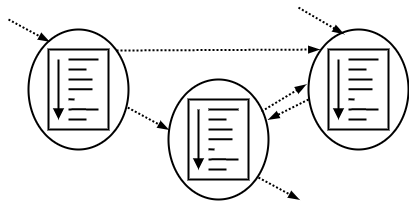
\includegraphics[width=0.55\textwidth]{img/03_proc.png}
\end{figure}

\end{frame}

%%%%%%%%%%%%%%%%%%%%%%%%%%%%%%%%%%%%%%%%%%%%%%%%%%%%%%%%%%%%
\begin{frame}
\frametitle{Rules for naming Identifiers}

\begin{itemize}
\item Identifiers \textcolor{red}{MUST} start with a letter or an underscore ($\_$).
\item Subsequent characters may be letter, digit, dollar sign(\$) or underscore,
\item Verilog does not restrict name length (but keep it short)
\item Tool or methodology may restrict name length
\item Identifiers are case sensitive
\begin{itemize}
	\item CNT, Cnt, cnt are all different legal names
\end{itemize}
\end{itemize}
\vfill
\textcolor{red}{*} Keywords are all lower-case.
\newline
\textcolor{red}{*} Built-in and user-defined system task and functions start with a dollar sign (\$). These are not user identifiers in the normal sense.

\end{frame}

%%%%%%%%%%%%%%%%%%%%%%%%%%%%%%%%%%%%%%%%%%%%%%%%%%%%%%%%%%%%
\begin{frame}
\frametitle{Escape Identifiers}

\begin{itemize}
\item An escaped identifier accepts any printable ASCII character in any position.
\item We can escape an identifier by using a backslash (\textbackslash) prefix and a whitespace (space, tab, newline) suffix. The backslash and whitespace are not part of the identifier.
\item Escaped identifiers exist to provide compatibility with tools and technology libraries. 
\item Some tools, for example, break vector variables into scalar variables that include their bracketed index in their name. The name must be escaped in order to allow the brackets.
\item Some libraries, start cell names with a digit to indicate number of inputs. The name must be escaped in order to allow initial digit.
\end{itemize}

\vfill

\textcolor{red}* Usually we shouldn't declare ourselves escaped identifiers because they make out code less readable.

\end{frame}

%%%%%%%%%%%%%%%%%%%%%%%%%%%%%%%%%%%%%%%%%%%%%%%%%%%%%%%%%%%%
\begin{frame}
\frametitle{Examples for Naming Identifiers}
\textcolor{red}{Not-Legal:}
\begin{itemize}
\item counter-1
\item 1\_counter
\item \$counter
\end{itemize}

\textcolor{green}{Legal:}
\begin{itemize}
\item counter\_1
\item counter\_1\_final\_final
\item counter\$
\end{itemize}

\textcolor{green}{Escaped:}
\begin{itemize}
\item \textbackslash counter-1
\item \textbackslash 1\_counter
\item \textbackslash \$counter[123]
\end{itemize}
\end{frame}

%%%%%%%%%%%%%%%%%%%%%%%%%%%%%%%%%%%%%%%%%%%%%%%%%%%%%%%%%%%%
\begin{frame}[fragile]
\frametitle{Rules for Comments and White Space}

\begin{itemize}
\item Single line comments starts with \textbackslash\textbackslash \ and ends with newline
\item A block comment starts anywhere with \textbackslash * and ends with *\textbackslash 
\end{itemize}
{\footnotesize%
\begin{Verbatim}[commandchars=\\\{\}, tabsize=2]
	\textcolor{blue}{\textbackslash\textbackslash This module ADDS perfectly!}
	\textcolor{purple}{module} adder (a, b, sel, sum, carry, y);
	\textcolor{purple}{input} a, b, sel; \textcolor{blue}{\textbackslash\textbackslash module inputs}
	\textcolor{purple}{output} \textcolor{blue}{\textbackslash* module outputs *\textbackslash} sum, carry, y;
\end{Verbatim}
}

\begin{itemize}
\item Verilog is free format language.
\item White space is needed only to separate some language tokens. We use additional white space to enhance readability
\end{itemize}

{\footnotesize%
\begin{Verbatim}[commandchars=\\\{\}, tabsize=2]
	\textcolor{purple}{assign} sum   = a ^ b;
	\textcolor{purple}{assign} carry = a & b;
\end{Verbatim}
}

\begin{itemize}
\item Use indentation to enhance readability (at least 2 space)
\end{itemize}

{\footnotesize%
\begin{Verbatim}[commandchars=\\\{\}, tabsize=2]
	\textcolor{purple}{always} @ *
		\textcolor{purple}{if} (sel == 1)
			y = b;
		\textcolor{purple}{else}
			y = a;
	...
\end{Verbatim}
}

\end{frame}


%%%%%%%%%%%%%%%%%%%%%%%%%%%%%%%%%%%%%%%%%%%%%%%%%%%%%%%%%%%%
\begin{frame}
\frametitle{Using Design Libraries}

Some Verilog tools use compilation libraries:
\begin{itemize}
\item A collection of already-compiled modules or primitives which are stored in file system and referred to by a library name.
\item Compiler places output in "WORK" library which is specified by the user.
\item Configuration in Verilog provides a prioritized list of libraries from which to bind compiled cell descriptions to cell instances.
\end{itemize}

\begin{figure}[H!]
    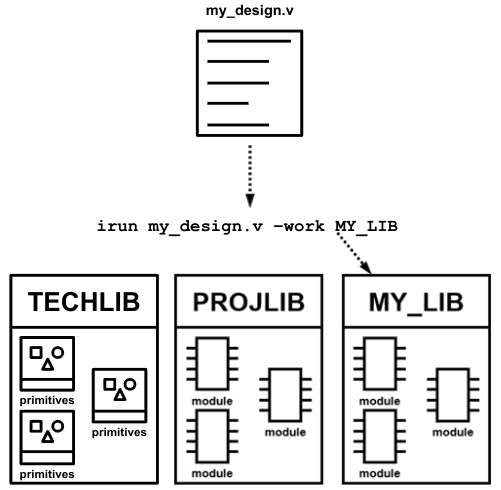
\includegraphics[width=0.45\textwidth]{img/03_design.png}
\end{figure}

\end{frame}

\note{

Simulating an HDL design and testbench is a process that first converts the source files into a binary form that the elaborator and simulator can recognize. This process of checking the syntax and producing the binary file is known as \textbf{compilation}.
\newline

Verilog tools that use libraries compile a design into a file system data structure known as a library. A vendor-specific mechanism selects one of those libraries as the \textbf{current working library}, and compilation by default places the results of compilation into that library. The elaboration process later selects design and testbench components from the libraries to construct the design and test configuration for simulation. 
}
%%%%%%%%%%%%%%%%%%%%%%%%%%%%%%%%%%%%%%%%%%%%%%%%%%%%%%%%%%%%
\begin{frame}
\frametitle{Compiling the design}

\begin{multicols}{2}
\begin{itemize}
\item Verilog compilation order is generally not important
\item Exception: compiler directievs
\begin{itemize}
	\item In source file(s)
	\item Tell compiler how to interpret subsequent code
	\item Not part of the design but affect how compiler creates the design
\end{itemize}
\end{itemize}

\vfill

\columnbreak

\begin{figure}[H!]
    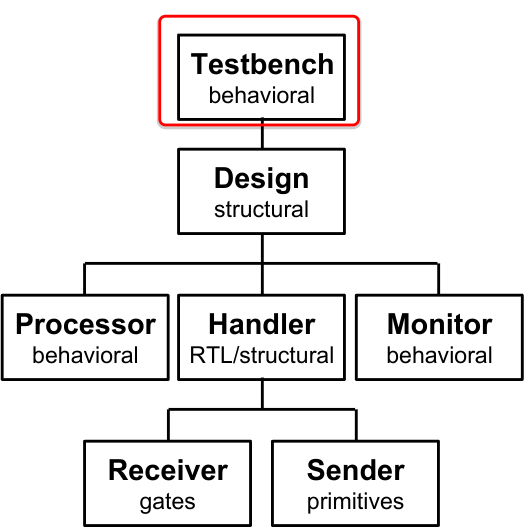
\includegraphics[width=0.45\textwidth]{img/03_compile.png}
\end{figure}
\end{multicols}

\end{frame}

\note{
Presented diagrams shows a complete hierarchical design with testbench.
\begin{itemize}
\item The behavioral testbench sits at the top level hierarchy. The testbench instantiates the design module and contains test code.
\item The structural design module instantiates the three primary design blocks and contains no design code of its own.
\begin{itemize}
	\item The behavioral processor module fully describes the processor functionality by itself.
	\item The behavioral monitor module fully describes the monitor functionality by itself.
	\item The RTL handler module partially describes the handler in synthesizable code and instantiates two sub-modules to complete the description. The receiver sub-module is an already synthesized netlist of ASIC vendor macros and the sender sub-module is a hand-crafted netlist of Verilog primitives.
\end{itemize}
\end{itemize}
}

\note{
You can normally compile these modules in any order. The exception is that if any of this file contains compile directives like \textbf{'ifdef, ifndef'} etc. that another file depends upon, then you must compile the files together and compile first the file containing the directives. \textcolor{red}{Creating such cross-file dependencies is considered bad practice.}

The elaborator later links together the compiled module descriptions to configure a design and testbench for simulation.
\newline

\textcolor{red}* Scope of compiler directive is from point read to wherever overriden or reset until the end of compilation session - across multiple files.
\newline

\textcolor{red}* Use compiler directives infrequently and carefully!!!  

}
%%%%%%%%%%%%%%%%%%%%%%%%%%%%%%%%%%%%%%%%%%%%%%%%%%%%%%%%%%%%
\begin{frame}
\frametitle{Module Summary}

We should now be able to use basic Verilog constructs to describe simple design.

This module very briefly introduced:
\begin{itemize}
\item Describing design modules (the \textbf{module} keyword)
\item Representing hierarchy (instantiation and port connection)
\item Describing module behavior (procedural blocks)
\begin{itemize}
	\item Synchronizing module behaviors (event controls)
	\item Communicating between behaviors (shared nets and variables)
\end{itemize}
\item Rules for identifiers, comments, white spaces
\item Compiling a design ("work" library and library map file)
\end{itemize}
\end{frame}


%%%%%%%%%%%%%%%%%%%%%%%%%%%%%%%%%%%%%%%%%%%%%%%%%%%%%%%%%%%%
\begin{frame}
\frametitle{Module Review}

\begin{enumerate}
\item What is the basic building block of a Verilog design?
\item How do Verilog procedures communicate or how is data passed between Verilog procedures?
\item When compiling a set of Verilog files, which is normally compiled first?
\end{enumerate}

\end{frame}

%%%%%%%%%%%%%%%%%%%%%%%%%%%%%%%%%%%%%%%%%%%%%%%%%%%%%%%%%%%%
\begin{frame}
\frametitle{Module Review - Solutions}

\begin{enumerate}
\item What is the basic building block of a Verilog design?
\begin{itemize}
	\item The Verilog basic building block is the module
\end{itemize}
\item How do Verilog procedures communicate or how is data passed between Verilog procedures?
\begin{itemize}
	\item Procedural blocks  by passing events, and by passing data via nets and shared variables informally called "signals" 
\end{itemize}
\item When compiling a set of Verilog files, which is normally compiled first?
\begin{itemize}
	\item This matters only if a later file utilizes compiler directives set by an earlier file
\end{itemize}
\end{enumerate}
\end{frame}

%%%%%%%%%%%%%%%%%%%%%%%%%%%%%%%%%%%%%%%%%%%%%%%%%%%%%%%%%%%%
\begin{frame}
\frametitle{Module Exercise}

Write a module instantiation statement to instantiate this module:
\begin{figure}[H!]
    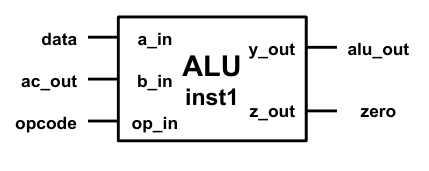
\includegraphics[width=0.5\textwidth]{img/03_module.png}
\end{figure}

\end{frame}

%%%%%%%%%%%%%%%%%%%%%%%%%%%%%%%%%%%%%%%%%%%%%%%%%%%%%%%%%%%%
\begin{frame}[fragile]
\frametitle{Module Exercise - Solution}

Write a module instantiation statement to instantiate this module:
\begin{figure}[H!]
    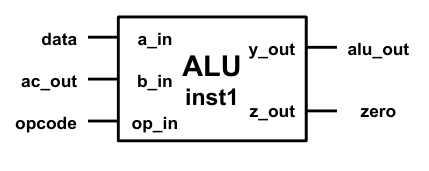
\includegraphics[width=0.5\textwidth]{img/03_module.png}
\end{figure}
Solution:
{\footnotesize%
\begin{Verbatim}[commandchars=\\\{\}, tabsize=2]
	ALU inst1 
	(
		.a_in  (data),
		.b_in  (ac_out),
		.op_in (opcode),
		.y_out (alu_out),
		.z_out (zero)
	);
\end{Verbatim}
}


\end{frame}

%%%%%%%%%%%%%%%%%%%%%%%%%%%%%%%%%%%%%%%%%%%%%%%%%%%%%%%%%%%%
\begin{frame}
\frametitle{Lab}

Lab 3-1: Modeling an Address Multiplexor
\begin{itemize}
\item Use basic Verilog constructs to describe a simple design.
\end{itemize}

\begin{figure}[H!]
    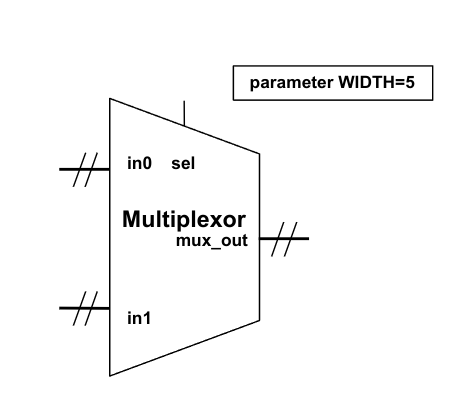
\includegraphics[width=0.5\textwidth]{img/03_lab.png}
\end{figure}

\end{frame}

%%%%%%%%%%%%%%%%%%%%%%%%%%%%%%%%%%%%%%%%%%%%%%%%%%%%%%%%%%%%
\begin{frame}
\frametitle{Test Your Understanding - 1}

We want to introduce a procedural block that executes repeatedly starting at simulation time 0. We use the keyword:
\begin{itemize}
\item[$\square$] procedure
\item[$\square$] always
\item[$\square$] process
\item[$\square$] initial
\item[$\square$] block
\end{itemize}

\end{frame}

%%%%%%%%%%%%%%%%%%%%%%%%%%%%%%%%%%%%%%%%%%%%%%%%%%%%%%%%%%%%
\begin{frame}
\frametitle{Test Your Understanding - 2}

We have declared the following variables. For which one or more will the compiler issue an error?
\begin{itemize}
\item[$\square$] 100\_CNT
\item[$\square$] \textbackslash \$100CNT
\item[$\square$] CNT\#100
\item[$\square$] \_CNT\$100
\item[$\square$] \$100CNT
\end{itemize}

\end{frame}

%%%%%%%%%%%%%%%%%%%%%%%%%%%%%%%%%%%%%%%%%%%%%%%%%%%%%%%%%%%%
\begin{frame}
\frametitle{Test Your Understanding - 3}

The basic elements to describe a design are (select one):
\begin{itemize}
\item[$\square$] modules
\item[$\square$] ports
\item[$\square$] macro modules
\item[$\square$] nets
\item[$\square$] primitives
\end{itemize}

\end{frame}

%%%%%%%%%%%%%%%%%%%%%%%%%%%%%%%%%%%%%%%%%%%%%%%%%%%%%%%%%%%%
\begin{frame}
\frametitle{Test Your Understanding - 4}

Which one or more space characters can be legally removed from this code:

always @ ( a,b ) if ( c ) d = e;
\newline
\begin{itemize}
\item[$\square$] space characters in \textcolor{blue}{"always @"}, \textcolor{blue}{") if ("}, and \textcolor{blue}{") d"}
\item[$\square$] space characters in \textcolor{blue}{"@ ( a,b )"}
\item[$\square$] space characters in \textcolor{blue}{"d = e;"}
\item[$\square$] space characters in \textcolor{blue}{"( c )"}
\end{itemize}

\end{frame}

%%%%%%%%%%%%%%%%%%%%%%%%%%%%%%%%%%%%%%%%%%%%%%%%%%%%%%%%%%%%
\begin{frame}
\frametitle{Test Your Understanding - 5}

Your RTL design modules intercommunicate by (select one):
\begin{itemize}
\item[$\square$] sending message packets to a global queue
\item[$\square$] notifying the testbench of internal event occurrence
\item[$\square$] dumping signal transition to a file
\item[$\square$] writing and reading ports externally interconnected by nets
\end{itemize}

\end{frame}

%%%%%%%%%%%%%%%%%%%%%%%%%%%%%%%%%%%%%%%%%%%%%%%%%%%%%%%%%%%%
\begin{frame}
\frametitle{Test Your Understanding Solution - 1}

We want to introduce a procedural block that executes repeatedly starting at simulation time 0. We use the keyword:
\begin{itemize}
\item[$\square$] procedure
\item[$\boxtimes$] always
\item[$\square$] process
\item[$\square$] initial
\item[$\square$] block
\end{itemize}

\end{frame}

%%%%%%%%%%%%%%%%%%%%%%%%%%%%%%%%%%%%%%%%%%%%%%%%%%%%%%%%%%%%
\begin{frame}
\frametitle{Test Your Understanding Solution - 2}

We have declared the following variables. For which one or more will the compiler issue an error?
\begin{itemize}
\item[$\boxtimes$] 100\_CNT
\item[$\square$] \textbackslash \$100CNT
\item[$\boxtimes$] CNT\#100
\item[$\square$] \_CNT\$100
\item[$\boxtimes$] \$100CNT
\end{itemize}

\end{frame}

%%%%%%%%%%%%%%%%%%%%%%%%%%%%%%%%%%%%%%%%%%%%%%%%%%%%%%%%%%%%
\begin{frame}
\frametitle{Test Your Understanding Solution - 3}

The basic elements to describe a design are (select one):
\begin{itemize}
\item[$\boxtimes$] modules
\item[$\square$] ports
\item[$\square$] macro modules
\item[$\square$] nets
\item[$\square$] primitives
\end{itemize}

\end{frame}

%%%%%%%%%%%%%%%%%%%%%%%%%%%%%%%%%%%%%%%%%%%%%%%%%%%%%%%%%%%%
\begin{frame}
\frametitle{Test Your Understanding Solution - 4}

Which one or more space characters can be legally removed from this code:

always @ ( a,b ) if ( c ) d = e;
\newline
\begin{itemize}
\item[$\boxtimes$] space characters in \textcolor{blue}{"always @"}, \textcolor{blue}{") if ("}, and \textcolor{blue}{") d"}
\item[$\boxtimes$] space characters in \textcolor{blue}{"@ ( a,b )"}
\item[$\boxtimes$] space characters in \textcolor{blue}{"d = e;"}
\item[$\boxtimes$] space characters in \textcolor{blue}{"( c )"}
\end{itemize}

\end{frame}

%%%%%%%%%%%%%%%%%%%%%%%%%%%%%%%%%%%%%%%%%%%%%%%%%%%%%%%%%%%%
\begin{frame}
\frametitle{Test Your Understanding Solution - 5}

Your RTL design modules intercommunicate by (select one):
\begin{itemize}
\item[$\square$] sending message packets to a global queue
\item[$\square$] notifying the testbench of internal event occurrence
\item[$\square$] dumping signal transition to a file
\item[$\boxtimes$] writing and reading ports externally interconnected by nets
\end{itemize}

\end{frame}
\end{document}
